%!TEX root = ../main.tex

\begin{IEEEbiography}[{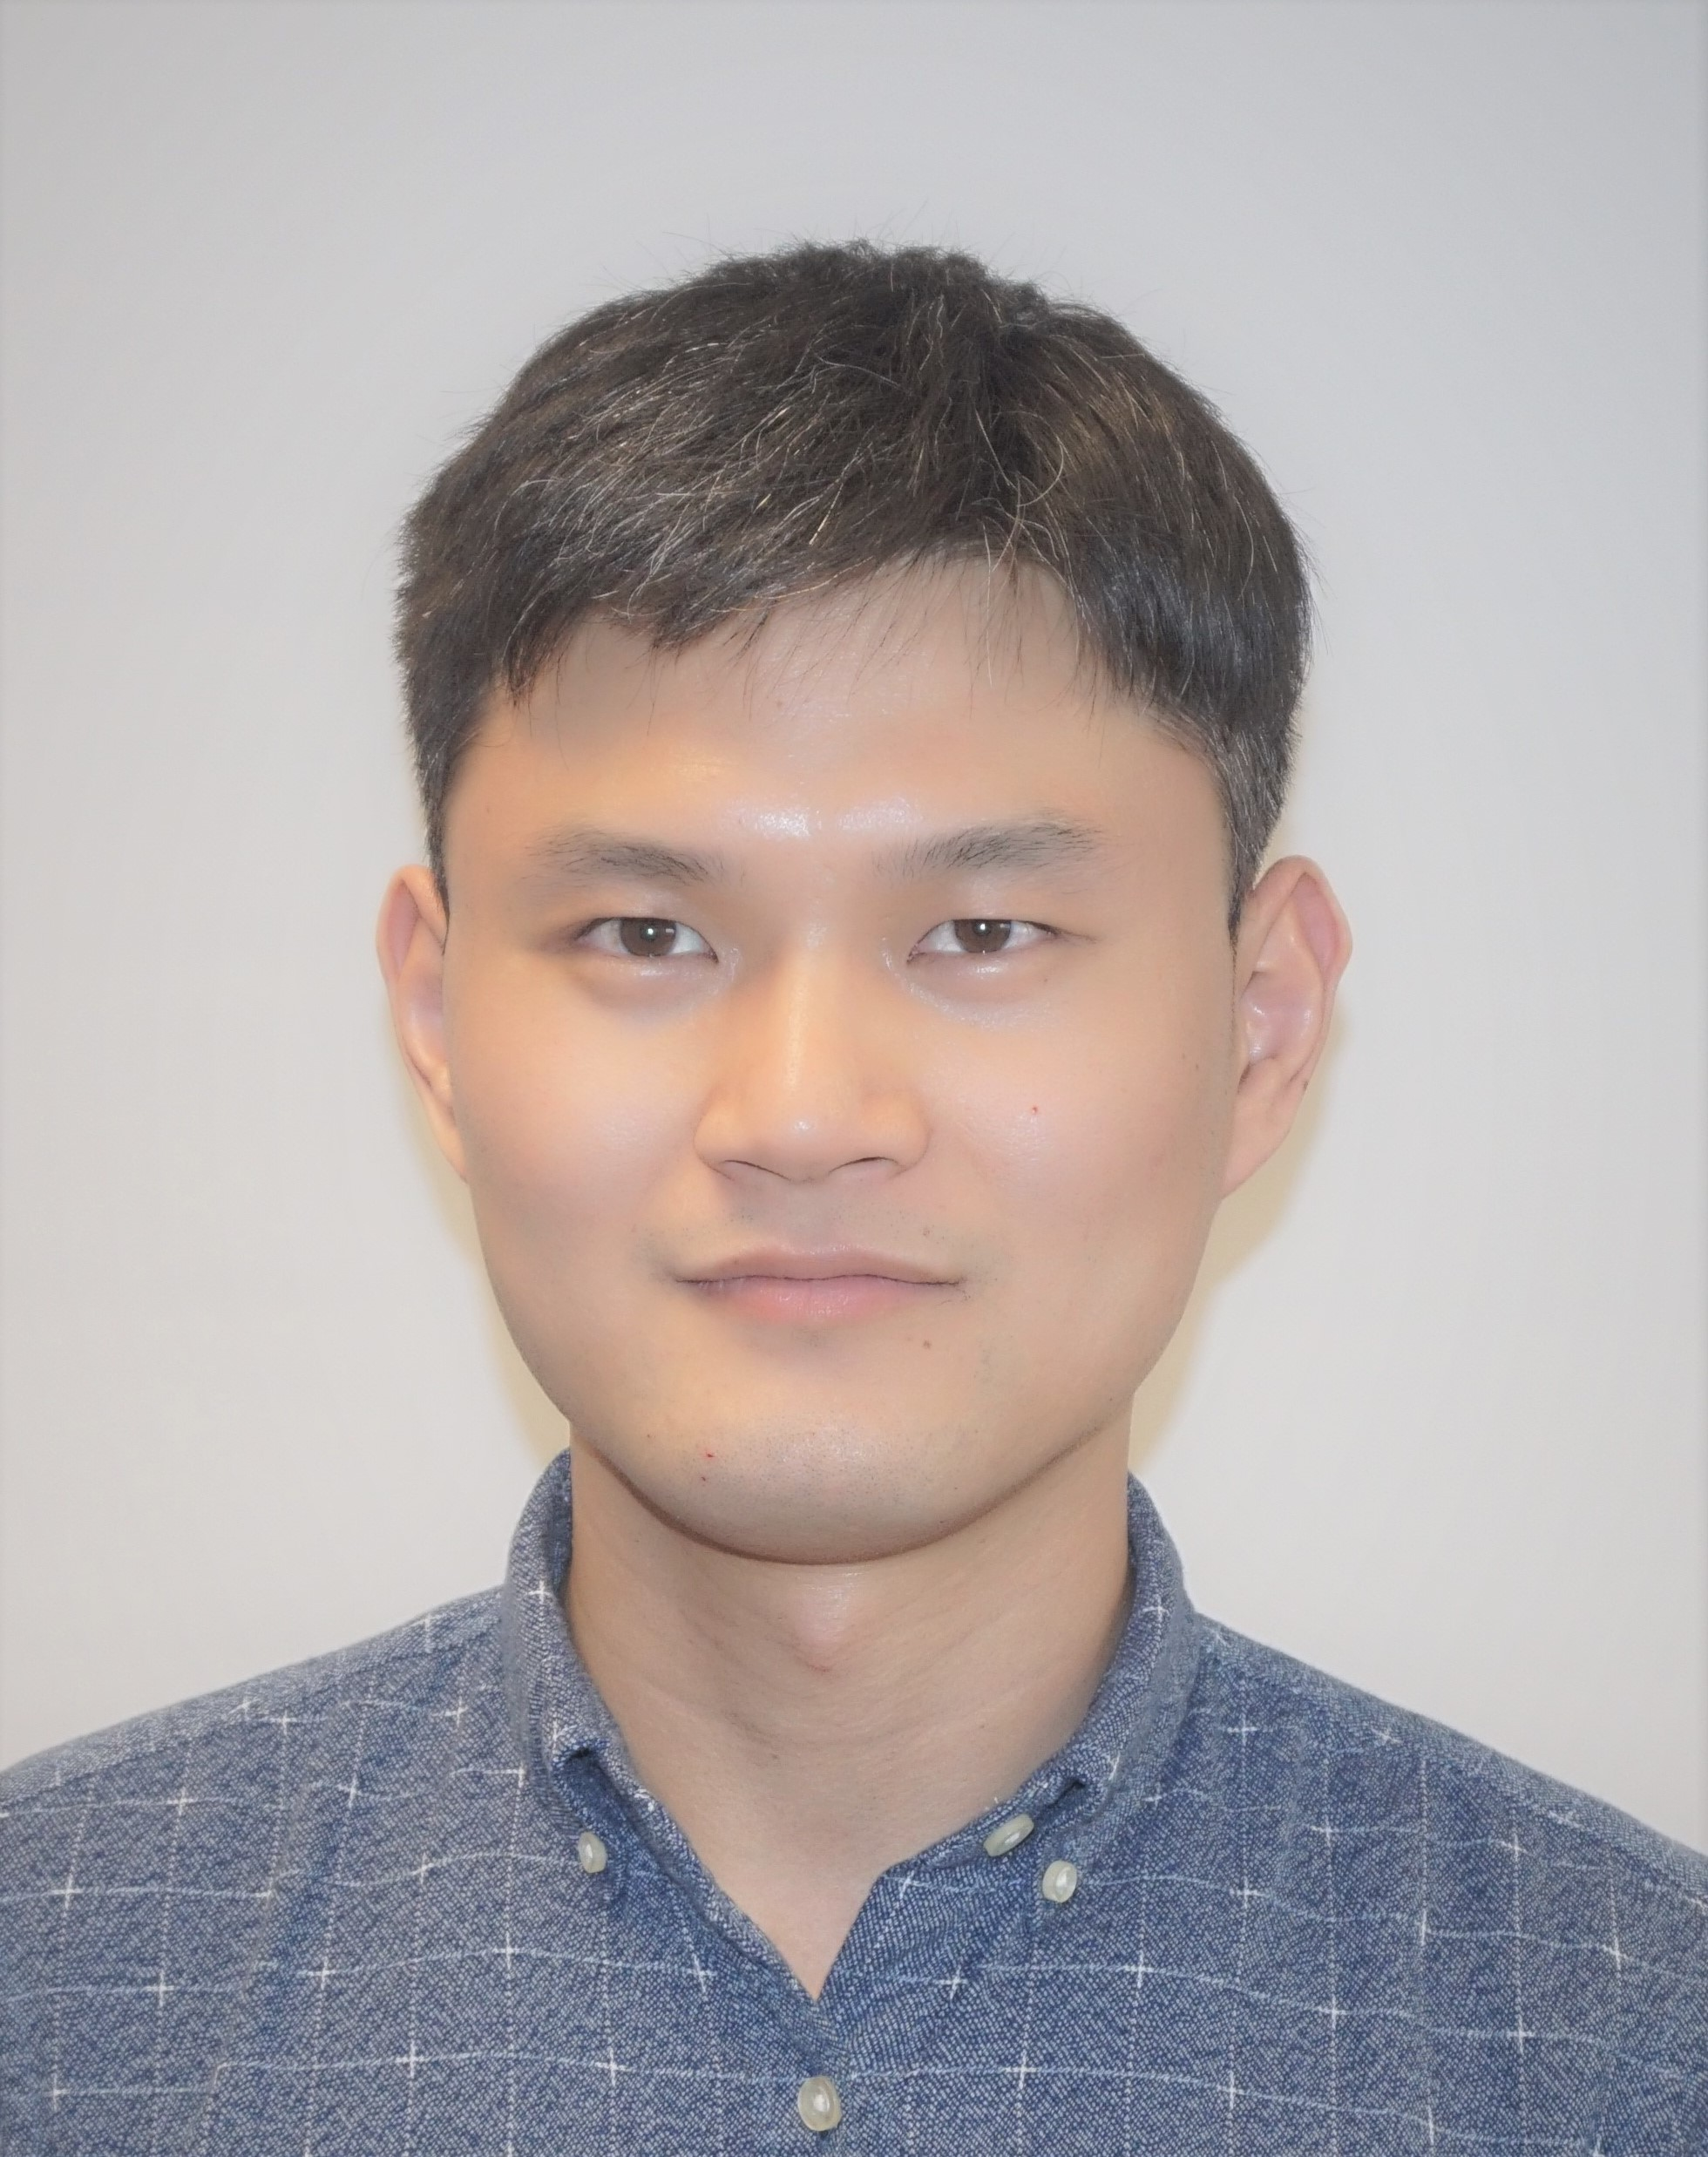
\includegraphics[width=1in,height=1.25in,clip,keepaspectratio]{appendix/yangyulin.jpg}}]{Yulin Yang}
received the B.Eng. degree in Mechanical Engineering from Shandong University, China, in 2009, and M.Sc. in Mechanical Engineering from Xi'an Jiaotong University, China in 2012. 
He is currently working toward a Ph.D. in department of Mechanical Engineering at University of Delaware. From 2012 to 2015, he was a Research \& Development Engineer at Siemens High Voltage Research Center in Shanghai, China. 
His research topics focus on visual inertial navigation, SLAM and nonlinear estimation. 
\end{IEEEbiography}




% if you will not have a photo at all:
\begin{IEEEbiography}[{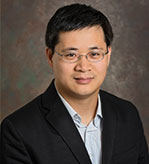
\includegraphics[width=1in,height=1.25in,clip,keepaspectratio]{appendix/Huang2014small.jpg}}]{Guoquan Huang}
received the B.Eng. in automation (electrical engineering) from University of Science and Technology Beijing,  China,  in  2002,  and  the  M.Sc.  and  Ph.D. in computer science from University of Minnesota--Twin Cities, Minneapolis, MN, USA, in 2009 and 2012, respectively. 


He  is  currently an Assistant Professor of Mechanical Engineering (ME), Electrical and Computer Engineering (ECE), and Computer and Information Sciences (CIS), at the University of Delaware (UD), Newark, DE, USA, where he is leading the Robot Perception and Navigation Group (RPNG). He also holds an Adjunct Professor position at the Zhejiang University, Hangzhou, China. He was a Senior Consultant (2016-2018) at the Huawei 2012 Laboratories and a Postdoctoral Associate (2012-2014) at MIT Computer Science and Artificial Intelligence Laboratory (CSAIL), Cambridge, MA. 
 %
His research interests  include sensing, localization, mapping, and perception of autonomous ground, aerial, and underwater robots. 


Dr. Huang received the 2006 Academic Excellence Fellowship from the University of Minnesota, the 2011 Chinese Government Award for Outstanding Self-Financed Students Abroad, the 2015 UD Research Award (UDRF), the 2016 NSF CRII Award, the 2017 UD Makerspace Faculty Fellow, the 2018 SATEC Robotics Delegation, the  2018 Google Daydream Faculty Research Award, and was the Finalist for the 2009 Best Paper Award from the Robotics: Science and Systems Conference (RSS).

\end{IEEEbiography}



